%%%%%%%%%%%%%%%%%%%%%%%%%%%%%%%%%%%%%%%%%
% MicromouseSymp Article
% LaTeX Template
% Version 0.2 (18/JAN/18)
% - added ORCID number
%
% Original author:
% Mathias Legrand (legrand.mathias@gmail.com) 
% With extensive modifications by:
% Antonio Valente (antonio.luis.valente@gmail.com)
%
% License:
% CC BY-NC-SA 3.0 (http://creativecommons.org/licenses/by-nc-sa/3.0/)
%
%%%%%%%%%%%%%%%%%%%%%%%%%%%%%%%%%%%%%%%%%

%----------------------------------------------------------------------------------------
%	PACKAGES AND OTHER DOCUMENT CONFIGURATIONS
%----------------------------------------------------------------------------------------

\documentclass[fleqn,10pt]{document} % Document font size and equations flushed left

\usepackage[english]{babel} % Specify a different language here - english by default
\usepackage{graphicx}

%----------------------------------------------------------------------------------------
%	ARTICLE INFORMATION
%----------------------------------------------------------------------------------------
\JournalInfo{University of Massachusetts Boston} % Journal information

\Archive{2020 Engineering Expo Proceedings} % Additional notes (e.g. copyright, DOI, review/research article)

\PaperTitle{Design and Validation of a Low Cost Magnetic Particle spectrometer} % Article title

\Authors{Apolinario Francisco, Jianjia Tan, Ryan Akerley} % Authors
\affiliation{Apolinario Francisco, Electrical Engineer, E-mail: \textit{Apolinario.franci001@umb.edu}} % Author affiliation
\affiliation{Jianjia Tan, Electrical Engineer, E-mail: \textit{jianjia.tan001@umb.edu}} % Author affiliation
\affiliation{Ryan Akerley, Computer Engineer, E-mail:
\textit{ryan.akerley002@umb.edu}}
\affiliation{\textbf{Advisor}: Dr.Alexey Tonyushkin, Research Assistant Professor, University of Massachusetts Boston} 

%\Keywords{Keyword1 --- Keyword2 --- Keyword3} % Keywords

%\newcommand{\keywordname}{Keywords} % Defines the keywords heading name

%----------------------------------------------------------------------------------------
%	ABSTRACT
%----------------------------------------------------------------------------------------

\Abstract{%
This paper presents a design and validation of a low cost  magnetic particle spectrometer, a technique used for the characterization of nanoparticles to use in a magnetic particle imaging research.
Magnetic particle imaging (MPI) is an emerging tracer-based molecular imaging technique which directly detects the intense magnetization of superparamagnetic iron oxide (SPIO), making it possible to  obtain a distribution of the tracer in the body. MPI provides high contrast-to-noise ratio signal with high sensitivity and zero tissue signal attenuation, and overall a better safety profile. Magnetic particle spectroscopy (MPS) is a technique that is used to characterize the SPIO, estimate the particle size distribution, to optimize the signal strength and resolution in the MPI research. 
Most MPS devices are extremely expensive (around \$70,000), therefore, few facilities have access to those devices. We  designed a low-cost MPS device using 3D-printed materials and off-the-shelf components for under \$1,000, while also creating an app for user interface. This app allows the data acquired to be saved and further processed on Excel or Matlab.
}%

\begin{document}
	
	\flushbottom % Makes all text pages the same height
	
	\maketitle % Print the title and abstract box
	
%	\tableofcontents % Print the contents section
	
	\thispagestyle{empty} % Removes page numbering from the first page
	
	%----------------------------------------------------------------------------------------
	%	ARTICLE CONTENTS
	%----------------------------------------------------------------------------------------
	
	\section{Introduction} % The \section*{} command stops section numbering
	%\addcontentsline{toc}{section}{Introduction} % Adds this section to the table of contents
	
    Magnetic particle imaging (MPI) is an emerging tracer-based molecular imaging technique which directly detects the intense magnetization of superparamagnetic iron oxide (SPIO), making possible to obtain a distribution of  tracers in the body. MPI could provide zero tissue signal attenuation, high contrast-to-noise ratio, high sensitivity, and a better safety profile \cite{p1}. The tracer has to be injected into the subject, but these tracers are natural (iron oxide), non-toxic and have been used to treat anemia and for magnetic resonance imaging (MRI) research in humans \cite{p2}\cite{p3}. The current MPI machine can only accommodate rodents, after proving the concept of MPI scanner, Dr. Alexey Tonyushkin intends to scale the device up to the size needed for human subject.
    Magnetic particle spectrometer (MPS) is used to characterize the magnetic particles, estimate particle size distribution, and optimize the signal strength and resolution in MPI research \cite{p4}. The objective of this project was to build an MPI  spectrometer to investigate the magnetic particles for Dr. Tonyushkin's MPI research. We provide a low-cost, robust, and user-friendly solution.
    
    One of the main part of the MPS project is a signal chain. The waveform for the transmit coil is generated on the Feather M4 Express microcontroller, a power amplifier is used to amplify the generated signal in order to provide the necessary current for the magnetic field generator coil. A Band Pass Filter (BPF) is used to filter out any harmonic distortion introduced by the power amplifier to ensure a pure sinusoidal waveform drives the transmit coil. The nanoparticles induce a signal in the receive coil and that signal is band-stop (BSF), amplified and digitized on the Data Acquisition system \cite{p5} \cite{p6}. 
MPI relies on magnetic nanoparticles tracers with certain properties in order to establish imaging protocols and accurately interpret data. The nanoparticles tracers need to be characterized to determine their response to the driving field of the MPI. A magnetic particle spectrograph is needed to establish the response to the driving field of varying concentrations of tracers, and to determine the properties of different tracers. This data will enable accurate readings from MPI data and also allow the selection of the best tracers for the required imaging task.
The software for the GUI and microcontroller will be released using the GNU General Public License (GPL) and source code placed on Github so that researchers in the field of MPI can use and further modify our designs to further their research.
 

\begin{figure*}[ht]\centering
\includegraphics[width=\linewidth]{ENGIN 492 Proceedings Template and Samples/Expo Proceedings LaTex Template/Design.png}
\caption{MPS System Diagram}
\label{fig:sytem}
\end{figure*}

	%This sample \cite{p3} file %\cite{grantseggbot} is intended to serve %as a ``starter file''
	%for Micromouse Symposium papers produced %under \LaTeX\ using
	%MicromouseSymp.cls version 0.1 and later.
	
	
	
	\section{Background}
	

	Currently there is only one company in Germany (Pure Devices) that design and manufacture MPS device, it cost about \$72,690 to buy the device and ship it to Boston. 
    The Pure Devices MPS Langevin model is used to do the characterization of contrast agents, it is also used to determine the mean size of particle and iron concentration of the sample. The frequency of the excitation field is 20kHz by default, the drive field can be set between 0 to 30mT, and the volume of the sample should be between 10 to 50$\mu$l with a test tube of 6mm diameter. The data acquired can be saved for further processing on Excel or Matlab \cite{p7}. It is powerful and has a GUI that is easy to control the device. It is a desired device except for the price. Also, the test tube size is fixed to 6mm, which is not convenient. Because of the limitations of the Pure devices MPS, Some universities have developed their own MPS \cite{p8}, we used those designs, to guide us to our own model and circuit design.
    The cost of design and produce a MPS device was around \$733.68 dollars and this device is going to be used primarily by Dr. Tonyushkin at the University of Massachusetts Boston.  
    \subsection{Global and Societal context}
    Since the first system was established and reported in 2005 by Philips Research Laboratories, MPI has emerged as a non-invasive tomographic technique that has proven useful in diagnostic imaging. MPS is a novel measurement method that closely relates to MPI \cite{p9} \cite{p10}.  The success of MPS will have an immediate impact on professor Tonyushkin MPI research project, the device will provide him the technology for evaluating the properties of nanoparticle traces,  and after more debugging and improvements on that device, the low cost version of MPS will provide more opportunities for researchers who need to use that into the future research on campus rather than buying expensive market products. 

MPI is a new technique and currently there are only few commercial companies developing imaging machine and it can only accommodate mice. Even though is not yet in clinical use it is very promising for several medical applications \cite{p11}, such as cerebral and cardiovascular flow, cancer detection and staging, therapeutic (stem) cell tracking to sites of pathology, real-time tracking of interventional instruments. There are couple solutions that help doctors with diagnostic imaging; techniques such as MRI, Computed Tomography (CT), and Positron emission Tomography (PET). Most of this solutions use Gadolinum (MRI), radioactive isotopes (PET) and iodine (CT), and in some of this techniques there is a risk of radiation exposure \cite{p12}. This techniques are also expensive and take a long time to get that image and the resolution is limited \cite{p12}. Most of the times doctors have to use a combination of this techniques to provide a full diagnostic analysis. MPI might provide a full diagnostic analysis in one single machine, reducing the overall
diagnostic duration. Overall it would reduce diagnostics
pathways and it would make easier and quicker for doctors to diagnose the diseases, consequently
reducing the amount of time that patients spend on hospital.
MPI is promises to be safer, cheaper and faster than current imaging techniques. It’s faster than MRI and it not use ionizing radiation like on CT scans and X-rays.

	\section{Design}
	\subsection{Hardware}
	
The hardware design of the MPS device mainly consists of three coils and two filters.
The core of the MPS device is a transmit coil, which is used for the excitation of the nanoparticles. It was designed in way that provides sufficient excitation field while minimizing power and current requirements; to avoid using active cooling the current should be kept below 10Amps. The transmit coil (figure 2) operates at a frequency of 25kHz and made using a 136mm long acrylic tube with an inner diameter of 63.5mm by winding 636 turns of 41/36 continuous litz wire, which is equivalent to an AWG \#20 single wire. Such coil is projected to generate a magnetic field of 30.4mT (equation 1) with an overall inductance of 50.3mH (equation 2), consisting of 6 layers and 106 turns per layer. We are going to validate the transmit coil by testing the magnetic field that the coil generates and  resistance of the coil, the coil should have low resistance. 

\begin{figure}[ht]\centering
    \includegraphics[width=\linewidth]{ENGIN 492 Proceedings Template and Samples/Expo Proceedings LaTex Template/Transmit coil.pdf}
    \caption{Transmit coil design}
    \label{fig:Transimit}
\end{figure}

\begin{equation}
    B = \frac{\mu_oNI}{l}
\end{equation}
%equation here 

\begin{equation}
	L = \mu_r\mu_0\frac{N^2A}{l}
	\label{eq:refname2}
\end{equation}

When calculating the magnetic field we used a wire size and current rating guide to find the wire gauge need \cite{p13}. This is important because it tells us how much current can run in a wire before melting the conductor or the wire insulation, for a maximum projected operating current of 4A the A.W.G is \#20.

\begin{figure}[ht]\centering
    \includegraphics[width=\linewidth]{ENGIN 492 Proceedings Template and Samples/Expo Proceedings LaTex Template/passfitler.png}
    \caption{Band-pass filter}
    \label{fig:filters bandpass}
\end{figure}

To ensure that the amplified  generated signal is purely sinusoidal,  we build a band-pass filter (figure 3) with a cut off frequency of 25kHz. The filter was made using polypropylene capacitors (for high power amplitude), and we build our own toroidal-shape 3D print indicators (L1 and L2, for the high current) they have an inner diameter of 50mm, outer diameter of 100mm and a height of 50mm.

\begin{figure}[ht]\centering
    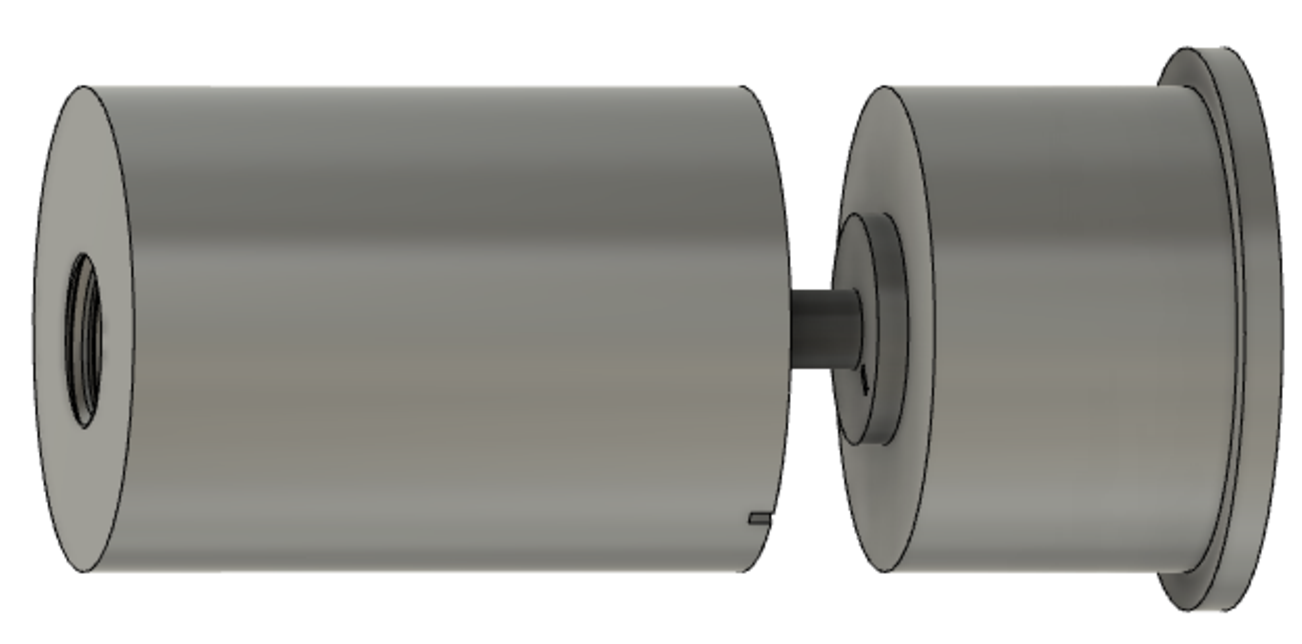
\includegraphics[width=\linewidth]{ENGIN 492 Proceedings Template and Samples/Expo Proceedings LaTex Template/Receiving.pdf}
    \caption{Receiving coil design}
    \label{fig:receving}
\end{figure}

\begin{figure}[ht]\centering
    \includegraphics[width=\linewidth]{ENGIN 492 Proceedings Template and Samples/Expo Proceedings LaTex Template/control.pdf}
    \caption{Control coil design}
    \label{fig:Control}
\end{figure}

The receive (figure 4) and control coils (figure 5) were made from 3D printed material (Nylon), both coils were design to be closer to the center of the transmit coil to achieve a more linear excitation field. The receive coil was design so it fits tighter inside the transmit coil to avoid components moving or unstable connection during the data acquisition process. To achieve maximum cancellation the number of turns in the receiving coils as to be the same as the number of turns in the control coil, but they should be winding in opposite direction. The receiving coil was made using 18mm long and by winding in a clockwise direction 20 turns of 160/44 litz wire which is equivalent to AWG \#22 single wire, with an inductance of 2.25 $\mu$H (equation 2). The receiving coil was built in a way that minimizes the distance between the coil and the sample, to maximize the sensitivity to the nanoparticle sample (The sample tube which will contain the nanoparticles has a diameter of 5 mm and a height 177.8mm. its located on the top of the receive coil to) and minimizing the feed trough due to the strong excitation field component.

The control coil sits in the excitation field coaxial with the transmit coil, in line with the receive coil but far enough from the sample so as not to pick up harmonics generated by the sample. The control coil is connected in series with the receive coil but at reverse polarity to the receive coil, so as to cancel out the excitation field while preserving the signal generated by the sample. The control coil is movable within the excitation field to adjust for maximum cancellation. To achieve maximum cancellation of the excitation field while minimizing cancellation of the signal requires very careful alignment of the control coil. Devising a mechanism that allows the coil to be adjusted when necessary, but that does not deviate from the desired setting once it has been achieved is crucial.
   
We also build a band-stop filter (figure 6) with a cut off frequency of 25kHz to achieve rejection of the drive component at the first harmonic. Since the signal current driving the receive coil is tiny we can use a regular ceramic capacitor and regular inductor from digikey. 
We are using copper shielding for the transmit coil, band-pass and band-stop filter to keep the internal circuit from some potential external hazard. The case should also provide EMI and RFI shielding, both to protect the receiving coil from extraneous noise that would affect accuracy, as well as containing the signal from the excitation field to protect other equipment in the lab.


\begin{figure}[ht]\centering
    \includegraphics[width=\linewidth]{ENGIN 492 Proceedings Template and Samples/Expo Proceedings LaTex Template/band-stop.png}
    \caption{Band-stop filter}
    \label{fig:filters bandstop}
\end{figure}

	\subsection{Software}
	The software to control the system consists of a cross-platform Graphical User Interface (GUI) app, written in Python, as well as the microcontroller software written in CircuitPython. The GUI app allows the user to easily automate driving the excitation field at multiple different power levels to collect data on the nonlinear response of the sample to different power levels. The app also displays data collected, and allows it to be exported in Comma Separated Value (CSV) format for manipulation and display in other software, such as Excel or Matlab.
	
	To operate the Spectrometer, the user enters the starting, ending, and step power levels as a percent of full power. The microcontroller then outputs the driving signal at each power level for 200ms and data is captured by the DAQ. The data is displayed in four graphs. Two graphs display the relative phase and amplitude, respectively, of the odd harmonics generated. The third graph shows the instantaneous magnetic moment of the sample graphed against time, while the fourth graph shows the magnetic moment of the sample graphed against the field strength of the driving field.
	
	The software is written in Python, an easy to learn and widely used programming language. The GUI is written using the TkInter package; a standard GUI library built on Tcl/Tk which is included with most distributions of Python. Additionally, the Matplotlib package is used for plotting of data. The software is open-source under the GNU General Public License (GPL) and will be made available on Github. These design decisions were made with the aim of allowing other researchers and students to use this system to further their research, as well as allowing them to improve and adapt the software to better meet their needs.
	
	The microcontroller used to generate the driving signal is the Feather M4 Express from Adafruit \cite{p14}. The M4 Express was chosen for its high-quality digital to analog converter (DAC) which, at a sampling rate of 64kHz and resolution of 16 bits, is able to generate the 25kHz signal for the drive coil. The microconroller is programmed in Circuitpython; a Python-derived language for embedded devices. The advantage of using Circuitpython is that, like Python, it is a simple language to learn. In addition, the microcontroller can be reprogrammed by attaching it to a computer by USB and editing the code.py file in a text editor; no other software is needed.
	
	

\subsection{Budget}
Figure eight show the budget breakdown, the cost of components and possible source for those components. 
	
	\begin{figure}[ht]
	    \centering
	    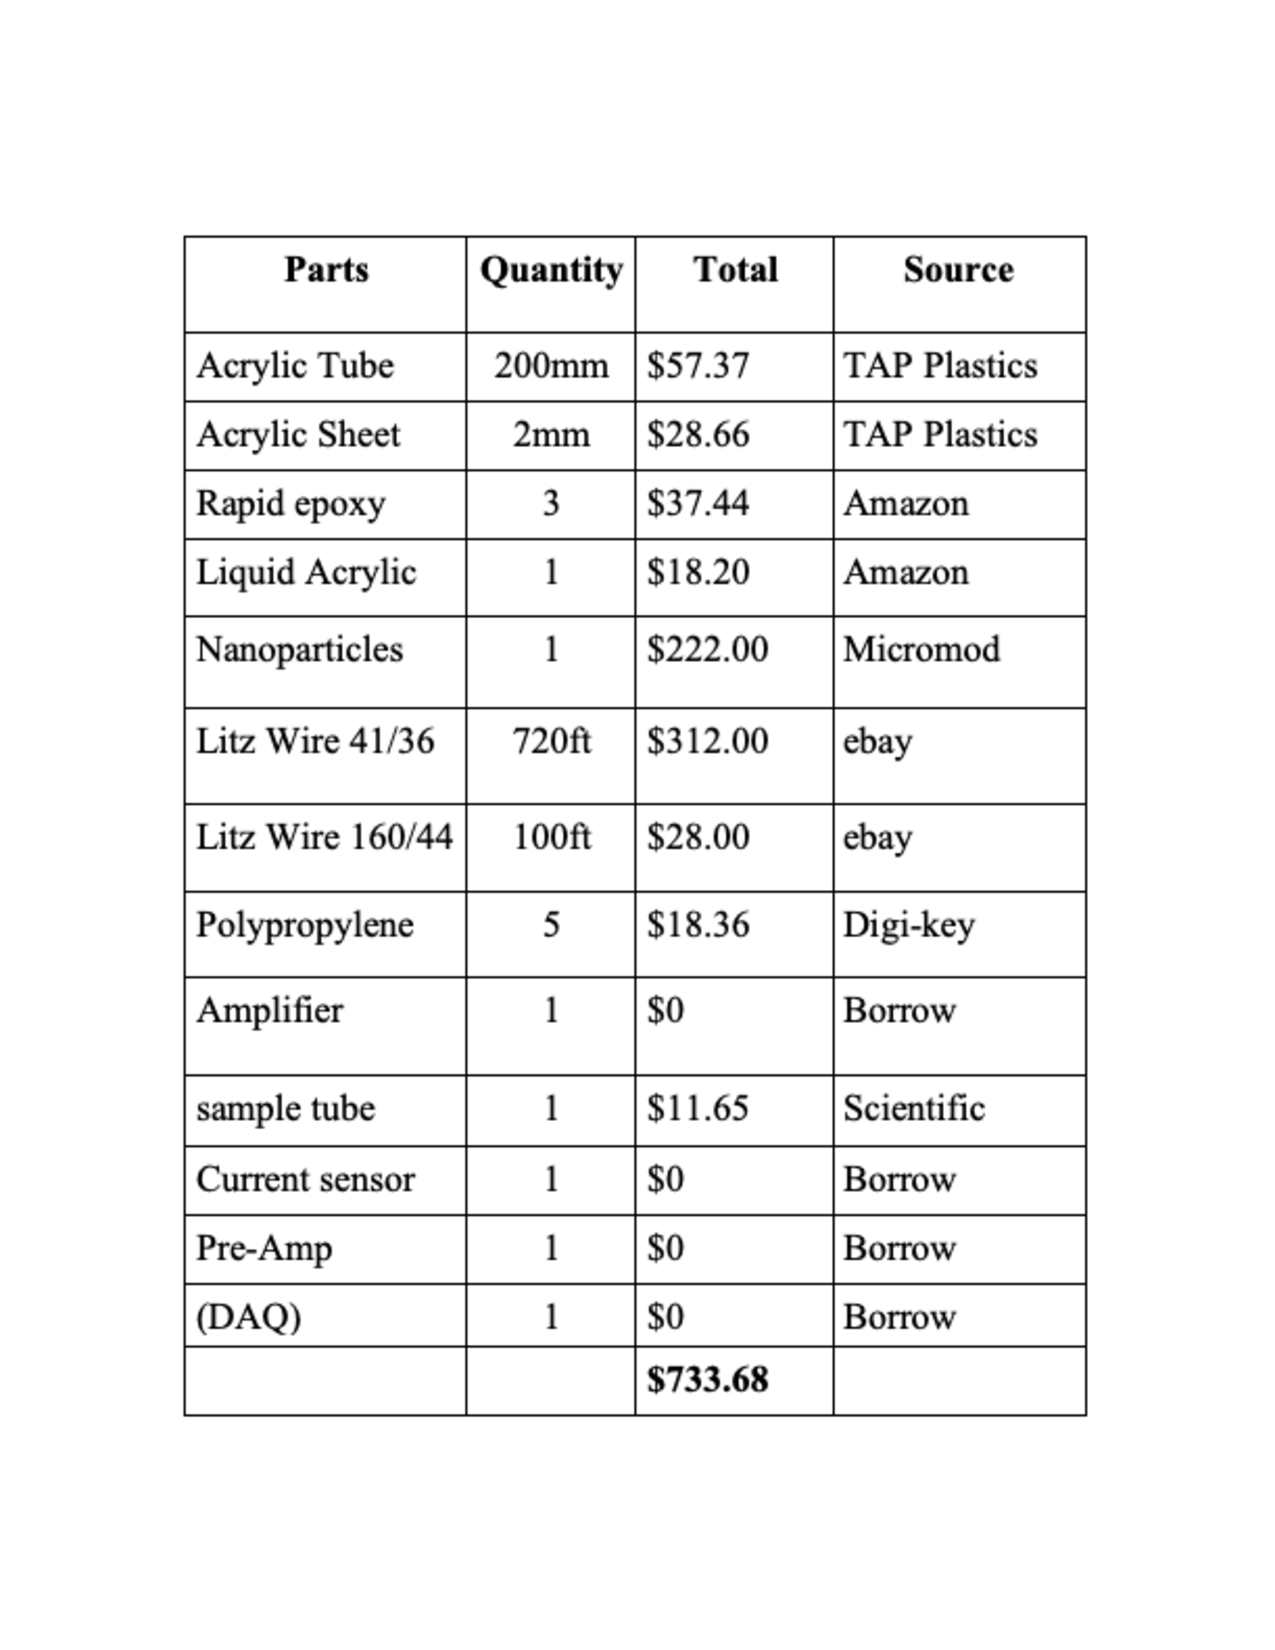
\includegraphics[width=\linewidth]{ENGIN 492 Proceedings Template and Samples/Expo Proceedings LaTex Template/budget.png}
	    \caption{Budget Breakdown}
	    \label{table:budget}
	\end{figure}
	
	\section{Results}
	\subsection{Hardware}
	
	\begin{figure}[ht]
	    \centering
	    \includegraphics[width=\linewidth]{ENGIN 492 Proceedings Template and Samples/Expo Proceedings LaTex Template/results .pdf}
	    \caption{Circuit of Band-stop filter and receive coil}
	    \label{fig:results}
	\end{figure}

We finished the hardware design of the MPS, we built the transmit coil, printed the receive and control coil, and band stop filter. The transmit  coil (figure 2) was hand built, by winding 636 turns of continuous litz wire. The coil is projected to generate a magnetic field of 30mT. We have assembled parts of the MPS hardware every component is fits nicely, which is important during data acquisition process. The control coil is connect to the band-stop filter to test the rejection of the drive component at the first harmonic, because of the lack of testing equipment available off campus we have not been able to test the magnetic field that transmit coil generates and the filters response. We used Spice based analog electronic circuit to simulate the the band-pass and band-stop filters and we notice that they removed very unwanted features from the signal.


\subsection{Software}

	\begin{figure}[ht]
	    \centering
	    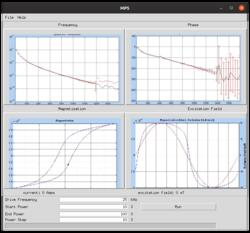
\includegraphics[width=\linewidth]{ENGIN 492 Proceedings Template and Samples/Expo Proceedings LaTex Template/app_screenshot.png}
	    \caption{user interface}
	    \label{fig:user_interface}
	\end{figure}
	
We created an app, written in Python, to control the spectrometer which has a GUI allowing the user to enter the parameters for testing and has an area to display the data collected. We also created software to control the microcontroller, written in CircuitPython, allowing it to generate the necessary driving signal at various power levels. The operation is as follows: The app running on the host computer communicates with the microcontroller using serial protocol over USB. When a run is initiated, the parameters are sent to the microcontroller, which then runs autonomously, generating the driving signal at the different power levels specified by the user. Running this way eliminates any lag or latency in communication between the host computer and the microcontroller.

While we were unable to test at the design frequency of 25kHz, the microcontroller shows stable frequency output at multiple power levels in the audio frequency range (specifically 440Hz, or A4). This was verified using a Peterson strobe tuner (normally used as a musical instrument tuner) which showed a steady 'A' when the microcontroller was outputting 440Hz. The GUI is able to take input parameters from the user and send them via serial protocol over USB to the connected microcontroller to generate driving frequencies at the different power levels selected by the user. We have applied the GPL open-source license to both the app and microcontroller software and hosted the software at \url{https://github.com/RyanAkerley/MPS}


	\section{Conclusion}
We have provided the details and characterization for the software and hardware use in creating a low cost magnetic particle spectrometer. more then 80\% of this project has been completed and the remaining 20\% (assembling and testing) will be done when it safe to use the school facility. 

	\phantomsection
	\section*{Acknowledgments} 
	
	\addcontentsline{toc}{section}{Acknowledgments} % Adds this section to the table of contents
	
We would like to acknowledge the Umass Boston Engineering Department for providing the funds and Resources.
We would to express our sincere thanks and appreciation to Dr. Alexey Tonyushkin for his assistance and for providing additional equipment. You supported us greatly and were always willing to help us.


	\phantomsection
	%\bibliographystyle{unsrt}
	\bibliographystyle{IEEEtran}
	\bibliography{document}

	
\end{document}